% -*- program: xelatex -*-

\documentclass[10pt
]{beamer}

% -----------------------------------------------------------------------------
\usetheme[numbering=fraction,
progressbar=frametitle,
% background=dark
]{metropolis}
% % use a heavier font for large room/underpowered projector
% \setsansfont[BoldFont={Fira Sans SemiBold}]{Fira Sans Book}

% % can use every beamer color theme!
% \usecolortheme{crane}
% \useoutertheme{metropolis}
% \useinnertheme{metropolis}
% \usefonttheme{metropolis}

% % or set colors by hand
% \setbeamercolor{...}{fg=...,bg=...}
% \setbeamercolor{progress bar}{...}
% \setbeamercolor{title separator}{...}
% \setbeamercolor{progress bar in head/foot}{...}
% \setbeamercolor{progress bar in section page}{...}

% -----------------------------------------------------------------------------
\usepackage{appendixnumberbeamer}  % do not count appendix slides, use \appendix to indicate 
% creative commons icons
\usepackage[scale=2]{ccicons} 
% fontawesome font/icons
\usepackage{fontspec}
\usepackage{fontawesome}      %
% Graphics4
\usepackage{graphicx}



%%% ---------------------------------------------------------------------------
\title{Statistical Eco(-toxico)logy}
\subtitle{Improving the Utilisation of Data for\\Environmental Risk Assessment}
\date{5\textsuperscript{th} January 2017}
\author{Eduard Sz\"{o}cs}



%%% ---------------------------------------------------------------------------
\begin{document}

%%% ------------------------------
\maketitle

\begin{frame}{Table of contents}
  \setbeamertemplate{section in toc}[sections numbered]
  \tableofcontents[hideallsubsections]
\end{frame}

%%% ---------------------------------------------------------------------------
\section{Environmental Risk Assessment (ERA)}


%%% ---------------------------------------------------------------------------
\section{Improving Statistics in ERA}

\begin{frame}
\frametitle{Ecotoxicology is not normal}

\end{frame}



\begin{frame}
\frametitle{A history of GLM (uncomprehensive)}

\end{frame}


\begin{frame}
\frametitle{Statistical Power is unacceptably low}

\end{frame}


\begin{frame}
\frametitle{Generalized Linear Models (GLM) can do better}

\end{frame}



\begin{frame}
\frametitle{What we learned}

\end{frame}


\begin{frame}
\frametitle{Where are we now?}

\end{frame}

%%% ---------------------------------------------------------------------------
\section{Exploring Monitoring Data for ERA}

\begin{frame}
\frametitle{Environmental Monitoring}

\end{frame}

\begin{frame}
\frametitle{Thresholds}

\end{frame}

\begin{frame}
\frametitle{Statistics with chemical measurements}

\end{frame}


\begin{frame}
\frametitle{Dynamics}

\end{frame}


\begin{frame}
\frametitle{Risks}

\end{frame}


\begin{frame}
\frametitle{What we learned}

\end{frame}

%%% ---------------------------------------------------------------------------
\section{Solutions for Linking Data in ERA}

\begin{frame}
\frametitle{Biologists \& Chemists face the same problems}

\end{frame}


\begin{frame}
\frametitle{Instead of wasting time...}

\end{frame}

\begin{frame}
\frametitle{webchem}
	\begin{center}
	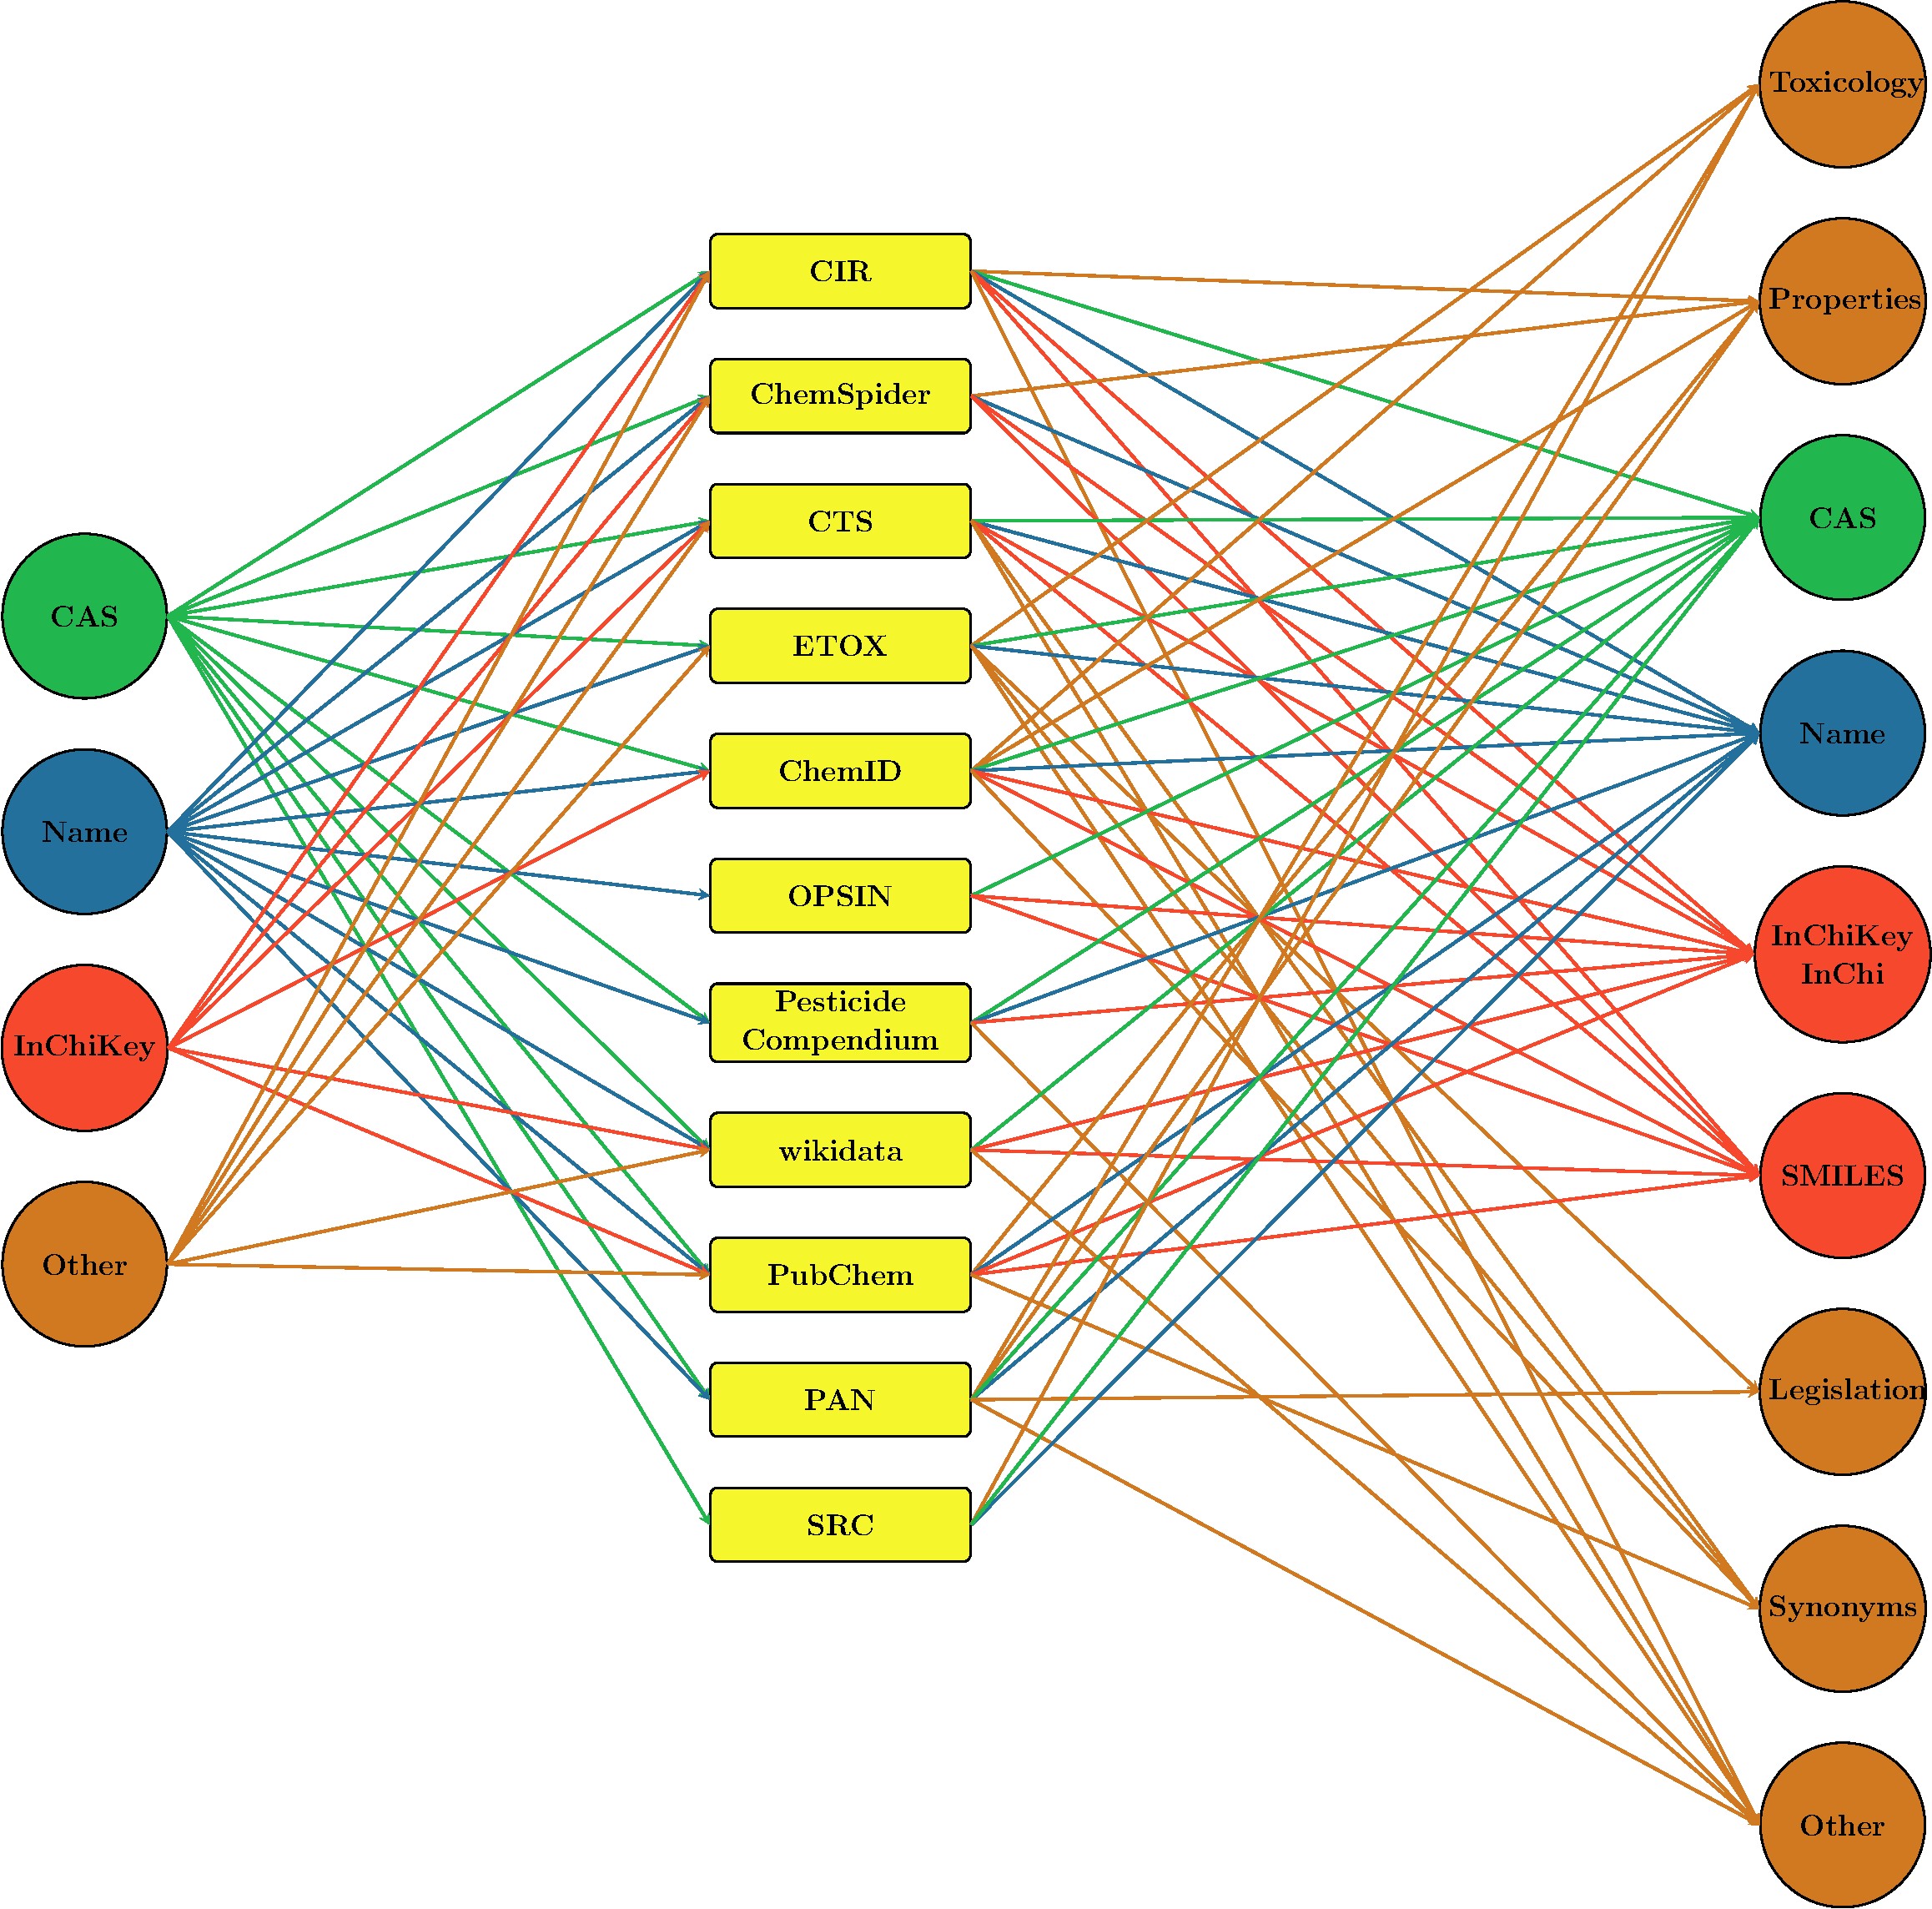
\includegraphics[width =.7\textwidth]{figs/sources_webchem.pdf} \\
	\end{center}

\end{frame}


\begin{frame}
\frametitle{Instead of wasting time...}

\end{frame}


%%% ---------------------------------------------------------------------------
\section*{Recap}

\begin{frame}
\frametitle{What we learned}
	\metroset{block=fill}
	\begin{exampleblock}{Improving Statistics in ERA}
		\textbf{Block content.}
	\end{exampleblock}

	\begin{exampleblock}{Exploring Monitoring Data for ERA}
		\textbf{Block content.}
	\end{exampleblock}

	\begin{exampleblock}{Solutions for Linking Data in ERA}
		\textbf{Use my R packages to save your time!}
	\end{exampleblock}


\end{frame}


%%% ---------------------------------------------------------------------------
%%% Final slide
\begin{frame}[standout]
	\frametitle{}

	\vspace{1em}
	\Huge{Statistical Ecotoxicology} \\[0.3em]
	\large{Improving the Utilisation of Data for \\ Environmental Risk Assessment} \\[1em]

	\normalsize
	Eduard Szöcs \\[3em]

	\faLaptop~~~\textbf{\href{http://edild.github.io/}{http://edild.github.io/ }}\\[.5em]
	\faTwitter~~~\textbf{\href{http://twitter.com/EduardSzoecs}{@EduardSzoecs}} 	\\[0.5em]
	\faGift~~~\textbf{\href{https://github.com/edild/talk_work2}{https://github.com/edild/phd\_defense}}\\[4em]

	\begin{center}\ccbysa\end{center} 

\end{frame}


\appendix

\begin{frame}
\frametitle{Statistics?}

\end{frame}


\begin{frame}
\frametitle{ZAGA what...?}

\end{frame}


\begin{frame}
\frametitle{Comparison with Stehle / Knauer?}

\end{frame}


\begin{frame}
\frametitle{webchem}

\end{frame}


\begin{frame}
\frametitle{taxize}

\end{frame}


\begin{frame}
\frametitle{ecology / biota?}

\end{frame}


% ------------------------------
\end{document}
